\section{Mereology}
\label{section:Mereology}

Mereology is the logical study on the semantics of parthood.
\textit{"As a formal theory, mereology is simply
an attempt to set out the general principles underlying the relationships between a whole and its constituent parts [...]"} \cite{DBLP:journals/dke/Varzi96}.
Achille C. Varzi describes a collection of formal theories, i.e. sets of distinct axioms, of mereology in \cite{DBLP:journals/dke/Varzi96}, which will be summarized in this section.

\ToDo{add SEP reference \cite{SEP:Mereology}}

\ToDo{add paragraph with applications of mereology in computer science \cite{w3org:OWLPartWhole}}

The first part of this section will just introduce the axioms of mereology.
Then, at the end of this section, we will use these axiom to build some of the theories described in \cite{DBLP:journals/dke/Varzi96}.
Note, that the terms relation, relationship and predicate may be used synonymously throughout this section.

\subsection{Parthood}
\label{subsection:Parthood}
First we define the intuitive notion of the parthood relationship:
\begin{definition}[$\partOf$]
Let $x$ and $y$ objects of interest.
We define:
\begin{align}
x \partOf y
:\Leftrightarrow
x \text{ is a constituent part of } y
\end{align}
\end{definition}
We further assume, that $\partOf$ satisfies the following properties:
\begin{align}
&\text{(P1)}
\qquad x \partOf x 
&\qquad \text{(Reflexivity)}
\\
&\text{(P2)}
\qquad x \partOf y \wedge y \partOf x \rightarrow x = y
&\qquad \text{(Antisymmetry)}
\\
&\text{(P3)}
\qquad x \partOf y \wedge y \partOf z \rightarrow x \partOf z
&\qquad \text{(Transitivity)}
\end{align}
Thus, $\partOf$ induces a partial order of things.

However, since the reflexive parthood may be to week for some cases, we also define a stricter, irreflexive parthood relationship as follows:
\begin{align}
x \properPartOf y
:\Leftrightarrow
x \partOf y \wedge \neg(y \partOf x)
&\qquad \text{(Proper Part)}
\label{definition:ProperPart}
\end{align}
Proper parthood induces a strict partial order of things.

\begin{figure}[h!]
\begin{center}
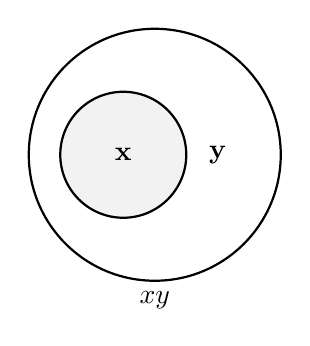
\begin{tikzpicture}[scale=0.8]
\draw[draw=black,thick](0,0)circle(2 and 2);
\draw[fill=gray!10,draw=black,thick](-0.5,0)circle(1 and 1);
\draw(-0.5,0)node{\textbf{x}};
\draw(1,0)node{\textbf{y}};
\node[anchor=north] at (current bounding box.south) {$x \properPartOf y$};
\end{tikzpicture}
\end{center}
{
\scriptsize 
This Venn-style diagram depicts a schematic illustration of Proper Part:
$x$ is certainly a part of $y$, however $y$ is not a part of $x$.
}
\caption{A schematic depiction of Proper Part}
\label{figure:SchematicProperPart}
\end{figure}


In addition to the relationships above we introduce the following predicates in order to provide a more concise notation:
\begin{align}
x \overlaps y
&:\Leftrightarrow
\exists z : z \partOf x \wedge z \partOf y
&\qquad \text{(Overlap)}
\label{definition:Overlap}
\\
x \underlaps y
&:\Leftrightarrow
\exists z : x \partOf z \wedge y \partOf z
&\qquad \text{(Underlap)}
\label{definition:Underlap}
\end{align}
Overlap models situations, where two things share at least on distinct part.
Underlap models situations, where two things are part of the same distinct thing.
Figure \ref{figure:SchematicOverlapAndUnderlap} illustrates both in a schematic fashion.

\begin{figure}[h!]
\begin{center}
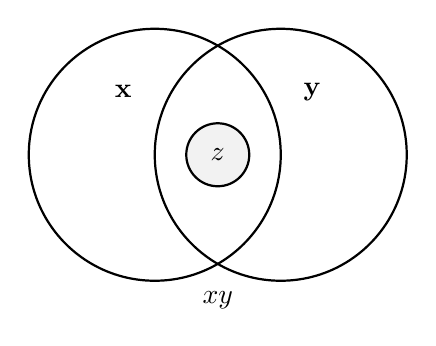
\begin{tikzpicture}[scale=0.8]
\draw[draw=black,thick](1,1)circle(2 and 2);
\draw[draw=black,thick](3,1)circle(2 and 2);
\draw[fill=gray!10,draw=black,thick](2,1)circle(0.5 and 0.5);
\draw(0.5,2)node{\textbf{x}};
\draw(3.5,2)node{\textbf{y}};
\draw(2,1)node{$z$};
\node[anchor=north] at (current bounding box.south) {$x \overlaps y$};
\end{tikzpicture}
\hspace*{5mm}
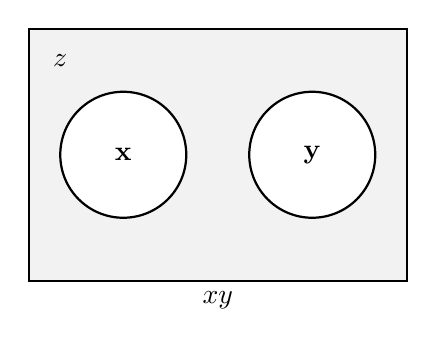
\begin{tikzpicture}[scale=0.8]
\draw[fill=gray!10,draw=black,thick](0,0)rectangle(6,4);
\draw[fill=white,draw=black,thick](1.5,2)circle(1 and 1);
\draw[fill=white,draw=black,thick](4.5,2)circle(1 and 1);
\draw(1.5,2)node{\textbf{x}};
\draw(4.5,2)node{\textbf{y}};
\draw(0.5,3.5)node{$z$};
\node[anchor=north] at (current bounding box.south) {$x \underlaps y$};
\end{tikzpicture}
\end{center}
{
\scriptsize 
These Venn-style diagrams depict schematic illustrations of Overlap \& Underlap:
\begin{itemize}
\item
$x \overlaps y$:
$x$ and $y$ share a distinct part $z$, which is emphasized as gray area.
\item
$x \underlaps y$:
$x$ and $y$ are both parts of $z$, which is emphasized as gray area.
\end{itemize}
}
\caption{A schematic depiction of Overlap \& Underlap}
\label{figure:SchematicOverlapAndUnderlap}
\end{figure}

\subsection{Identity \& Equality}
\ToDo{Define and outline Identity/Equality. Note seems to be some problems with mereological equality of words, see \cite{SEP:Mereology}}
\begin{align}
x = y
:\Leftrightarrow
x \partOf y \wedge y \partOf x
\qquad \text{(Identity)}
\end{align}

\noindent
The following equivalence for identity should also hold:
\begin{align}
x = y
\Leftrightarrow
x \partOf y \wedge y \partOf x
\Leftrightarrow
\forall z (z \partOf x \leftrightarrow z \partOf y)
\end{align}
Proof could look as follows:
\begin{align*}
&\forall z (z \partOf x \leftrightarrow z \partOf y)
\\&\Leftrightarrow
\forall z
((\neg(z \partOf x) \wedge \neg(z \partOf y)) \vee (z \partOf x \wedge z \partOf y))
\\&\text{extend the forumlar with self-conjunction:} a \wedge a
\\&\Leftrightarrow
\forall u
((\neg(u \partOf x) \wedge \neg(u \partOf y)) \vee (u \partOf x \wedge u \partOf y))
\\&\quad\wedge
\forall v
((\neg(v \partOf x) \wedge \neg(v \partOf y)) \vee (v \partOf x \wedge v \partOf y))
\\&\text{because of all-quantifaction the formular also holds for u := x and v := y}
\\&\Leftrightarrow
((\neg(x \partOf x) \wedge \neg(x \partOf y)) \vee (x \partOf x \wedge x \partOf y))
\\&\quad\wedge
((\neg(y \partOf x) \wedge \neg(y \partOf y)) \vee (y \partOf x \wedge y \partOf y))
\\&\text{reflixivness eliminates some terms}
\\&\Leftrightarrow
((false \wedge \neg(x \partOf y)) \vee (true \wedge x \partOf y))
\\&\quad\wedge
((\neg(y \partOf x) \wedge false) \vee (y \partOf x \wedge true))
\\&\Leftrightarrow
false \vee x \partOf y \wedge false \vee y \partOf x
\\&\Leftrightarrow
x \partOf y \wedge y \partOf x
\\&\Leftrightarrow
x = y
\end{align*}

\subsection{Supplementation}
\label{subsection:Supplementation}
The fourth axiom, which can be assumed in an universe described by means of mereology, is the supplementation axiom.
It models the effects of situations more precisely, where one thing is not part of another.
Namely, if this is the case, a third thing may exist, which is part of the former but not part of the latter.
\begin{align}
&\text{(P4)}
\qquad
\neg(x \partOf y) \rightarrow \exists z (z \partOf x \wedge \neg(z \overlaps y))
\end{align}
The supplementation axiom reads:
If a thing $x$ is not part of another thing $y$, then at least one part of $x$ does not share further parts with $y$.
Figure \ref{figure:SupplementaitonAxiomExample} depicts a schematic example of the supplementation axiom.

\begin{figure}[h!]
\begin{center}
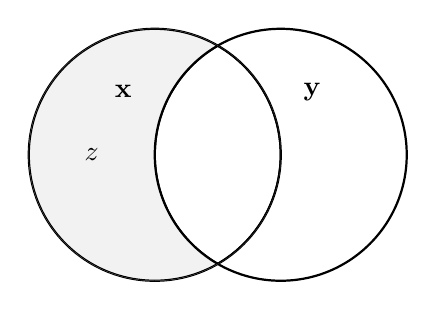
\begin{tikzpicture}[scale=0.8]
\draw[draw=black,thick](1,1)circle(2 and 2);
\draw[draw=black,thick](3,1)circle(2 and 2);
\scope
\clip(1,1)circle(2 and 2);
\draw[fill=gray!10,draw=black,thick, even odd rule]
(1,1)circle (2 and 2)
(3,1)circle(2 and 2);
\endscope
\draw(0.5,2)node{\textbf{x}};
\draw(3.5,2)node{\textbf{y}};
\draw(0,1)node{$z$};
\end{tikzpicture}
\end{center}
{
\scriptsize 
This Venn-style diagram exemplifies the supplementation axiom:
$x$ is not part of $y$.
$z$ is emphasized as gray area.
$x$ contains $z$, but $z$ shares no further parts with $y$.
}
\caption{A schematic example of the Supplementation Axiom}
\label{figure:SupplementaitonAxiomExample}
\end{figure}

%\usetikzlibrary{calc}
%\begin{tikzpicture}[scale=0.8]
%\draw(4,3)circle(5 and 3)node(A){Text A};
%\draw(8,6)circle(5 and 3)node(B){Text B};
%\draw(10,2.5)circle(5 and 3)node(C){Text C};
%\begin{scope}
%\clip(4,3)circle(5 and 3);
%\clip(8,6)circle(5 and 3);
%\clip(10,2.5)circle(5 and 3);
%\filldraw[yellow!80](0,0)rectangle(10,10);
%\end{scope}
%\node at ($0.33*(A)+0.33*(B)+0.33*(C)$){Text M};
%\end{tikzpicture}

\ToDo{add paragraph explaining "strong" and "weak" supplementation}

One can also observe from figure \ref{figure:SupplementaitonAxiomExample}, that the supplementation axiom can be interpreted as analogue to set-theoretic difference.

\subsection{Sum, Product \& Difference}
\label{subsection:SumProductAndDifference}
The next three axioms allow for the notions of sum, product and difference in a mereological context.

\subsubsection{Sum}
The fifth axiom, which can be assumed in an universe described by means of mereology, is the sum axiom.
It models the intuitive notion, where all parts of one thing and all parts of another thing are exactly the constituent parts of a third thing.

\begin{align}
&\text{(P5)}
\quad
&\begin{split}
&x \underlaps y 
\\&\rightarrow
\exists z \forall w (w \overlaps z \leftrightarrow (w \overlaps x \vee w \overlaps y))
\end{split}
\label{axiom:Sum}
\end{align}
The sum axiom reads:
If things $x$ and $y$ are two parts of the same thing, then another thing $z$ exist, which only shares parts with things, which in turn share parts with $x$ or $y$.
Then $z$ can be interpreted as the sum of $x$ and $y$.
This notion is captured by following definition of the term $z = x + y$:
\begin{align}
z = x + y
:\Leftrightarrow
\forall w (w \overlaps z \leftrightarrow (w \overlaps x \vee w \overlaps y))
\label{definition:Sum}
\end{align}
Figure \ref{figure:SumAxiomExample} depicts a schematic example of the sum axiom.
\begin{figure}[h!]
% http://www.texample.net/tikz/examples/set-operations-illustrated-with-venn-diagrams/
\begin{center}
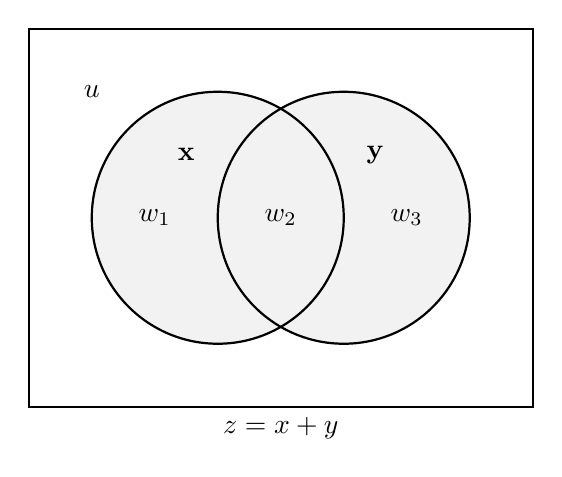
\begin{tikzpicture}[scale=0.8]
\draw[draw=black,thick](-2,-2) rectangle (6,4);
\draw[fill=gray!10,draw=black,thick]
(1,1)circle(2 and 2)
(3,1)circle(2 and 2);
\draw(0.5,2)node{\textbf{x}};
\draw(3.5,2)node{\textbf{y}};
\draw(-1,3)node{$u$};
\draw(0,1)node{$w_1$};
\draw(2,1)node{$w_2$};
\draw(4,1)node{$w_3$};
\node[anchor=north] at (current bounding box.south) {$z = x + y$};
\end{tikzpicture}
\end{center}
{
\scriptsize 
This Venn-style diagram exemplifies the sum axiom:
$x$ and $y$ are part of $u$.
$z = x + y$ is emphasized as gray area.
All $w_i$ share parts with $z$, if and only if they share parts with $x$ or $y$.
}
\caption{A schematic example of the Sum Axiom}
\label{figure:SumAxiomExample}
\end{figure}

One can also observe similarities between the sum axiom and set-theoretic union from figure \ref{figure:SumAxiomExample} and the definition \ref{definition:Sum}.

\subsubsection{Product}
The sixth axiom, which can be assumed in an universe described by means of mereology, is the product axiom.
It models the intuitive notion, where all things, which are parts of two things at the same time, are exactly the constituent parts of a third thing.
\begin{align}
&\text{(P6)}
\quad
&\begin{split}
&x \overlaps y 
\\&\rightarrow
\exists z \forall w (w \partOf z \leftrightarrow (w \partOf x \wedge w \partOf y))
\end{split}
\label{axiom:Product}
\end{align}
The sum axiom reads:
If things $x$ and $y$ share at least one part, then another thing $z$ exists, which only consists of parts, which in turn are parts of $x$ and $y$ at the same time.
Then $z$ can be interpreted as the product of $x$ and $y$.
This notion is captured by the following definition of the term $z = x \cdot y$:
\begin{align}
z = x \cdot y
:\Leftrightarrow
\forall w (w \partOf z \leftrightarrow (w \partOf x \wedge w \partOf y))
\label{definition:Product}
\end{align}
Figure \ref{figure:ProductAxiomExample} depicts a schematic example of the product axiom.

\begin{figure}[h!]
\begin{center}
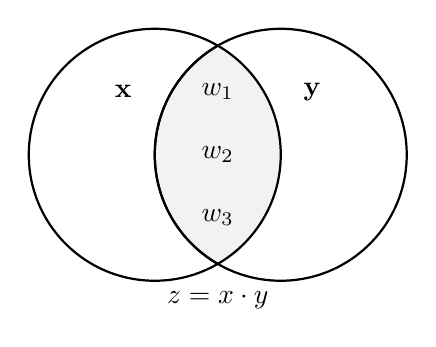
\begin{tikzpicture}[scale=0.8]
\scope
\clip(1,1)circle(2 and 2);
\fill[fill=gray!10,draw=black,thick](3,1)circle(2 and 2);
\endscope
\draw[draw=black,thick](1,1)circle(2 and 2);
\draw[draw=black,thick](3,1)circle(2 and 2);
\draw(0.5,2)node{\textbf{x}};
\draw(3.5,2)node{\textbf{y}};
\draw(2,2)node{$w_1$};
\draw(2,1)node{$w_2$};
\draw(2,0)node{$w_3$};
\node[anchor=north] at (current bounding box.south) {$z = x \cdot y$};
\end{tikzpicture}
\end{center}
{
\scriptsize 
This Venn-style diagram exemplifies the product axiom:
$x$ and $y$ share arts.
$z = x \cdot y$ is emphasized as gray area.
All $w_i$ are part of $z$, if and only if they are part of $x$ and $y$.
}
\caption{A schematic example of the Product Axiom}
\label{figure:ProductAxiomExample}
\end{figure}

One can also observe similarities between the sum axiom and set-theoretic intersection from figure \ref{figure:ProductAxiomExample} and the definition \ref{definition:Product}.

\subsubsection{Difference}
The seventh axiom, which can be assumed in an universe described by means of mereology, is the difference axiom.
It models the intuitive notion, where things may be split, so that their constituent parts are regrouped into disjoint things, which share no parts.
\begin{align}
&\text{(P7)}
\quad
&\begin{split}
&\exists z (z \partOf x \wedge \neg(z \overlaps y))
\\&\rightarrow
\exists z \forall w (w \partOf z \leftrightarrow (w \partOf x \wedge \neg(w \overlaps y)))
\end{split}
\label{axiom:Difference}
\end{align}
The difference axiom reads:
If for things $x$ and $y$ a supplementary thing exists, which is part of $x$, but shares no parts with $y$, then another thing $z$ exists, consisting of parts, which are also part of $x$, but share no parts with $y$.
Then $z$ can be interpreted as the difference between $x$ and $y$, in that order.
This notion is captured by the following definition of the term $z = x - y$:
\begin{align}
z = x - y
:\Leftrightarrow
\forall w (w \partOf z \leftrightarrow (w \partOf x \wedge \neg(w \overlaps y)))
\label{definition:Difference}
\end{align}
Figure \ref{figure:DifferenceAxiomExample} depicts a schematic example of the difference axiom.

\begin{figure}[h!]
\begin{center}
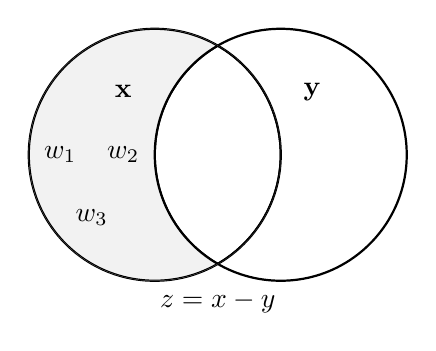
\begin{tikzpicture}[scale=0.8]
\draw[draw=black,thick](1,1)circle(2 and 2);
\draw[draw=black,thick](3,1)circle(2 and 2);
\scope
\clip(1,1)circle(2 and 2);
\draw[fill=gray!10,draw=black,thick, even odd rule]
(1,1)circle (2 and 2)
(3,1)circle(2 and 2);
\endscope
\draw(0.5,2)node{\textbf{x}};
\draw(3.5,2)node{\textbf{y}};
\draw(-0.5,1)node{$w_1$};
\draw(0.5,1)node{$w_2$};
\draw(0,0)node{$w_3$};
\node[anchor=north] at (current bounding box.south) {$z = x - y$};
\end{tikzpicture}
\end{center}
{
\scriptsize 
This Venn-style diagram exemplifies the difference axiom:
$x$ is not part of $y$ and parts of $x$ exists, which do not share parts with $y$.
$z = x - y$ is emphasized as gray area.
All $w_i$ are part of $z$, if and only if they are part of $x$ and do not share further parts with $y$.
}
\caption{A schematic example of the Difference Axiom}
\label{figure:DifferenceAxiomExample}
\end{figure}

One can also observe again similarities between the sum axiom and set-theoretic difference from figure \ref{figure:DifferenceAxiomExample} and the definition \ref{definition:Difference}.

\ToDo{Outline dependencies with supplementation axiom}

\subsection{Universal Top, Complement \& Bottom}
\label{subsection:UniversalTopComplementAndBottom}
The sum axiom (P5) at \ref{axiom:Sum} gives immediate rise to the idea, that all things can be summed up to an universal thing and all things are part of it.
This notion is captured by the top axiom:
\begin{align}
&\exists \top \forall x (x \partOf \top)
&\qquad \text{(Top)}
\label{axiom:Top}
\end{align}
Having an universe also facilitates the definition of a universal or absolute complement:
\begin{align}
&\complementOf{x} := \top - x
&\qquad \text{(Complement)}
\label{definition:Complement}
\end{align}
Figure \ref{figure:SchematicUniversalTopAndComplement} depicts a schematic illustration of an universal top and a complement.

\begin{figure}[h!]
\begin{center}
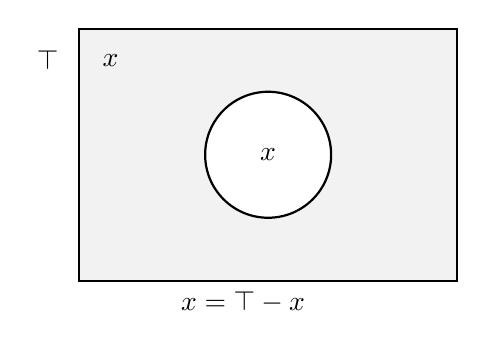
\begin{tikzpicture}[scale=0.8]
\draw[fill=gray!10,draw=black,thick](0,0)rectangle(6,4);
\draw[fill=white,draw=black,thick](3,2)circle(1 and 1);
\draw(3,2)node{$x$};
\draw(0.5,3.5)node{$\complementOf{x}$};
\draw(-0.5,3.5)node{$\top$};
\node[anchor=north] at (current bounding box.south) {$\complementOf{x} = \top - x$};
\end{tikzpicture}
\end{center}
{
\scriptsize 
This Venn-style diagram illustrates universal top and a complement:
Top $\top$ is the rectangle containing everything.
The complement $\complementOf{x}$ of $x$ is emphasized as gray area.
}
\caption{A schematic illustration of Universal Top \& Complement}
\label{figure:SchematicUniversalTopAndComplement}
\end{figure}

An universal top renders the underlap relationship as defined at \ref{definition:Underlap} trivially true, thus the mereological sum of two things as defined at \ref{definition:Sum} can never be undefined.
In an algebraic sense, an universal top also provides an absorbing element for mereolgical sum and a neutral element for the mereoligcal product as defined at \ref{definition:Product}:
\begin{align}
\top &= \top + x = x + \top
\\
x &= \top \cdot x = x \cdot \top
\end{align}

Properties of the mereological complement can in part be observed from figure \ref{figure:SchematicUniversalTopAndComplement}.
Obviously, in addition to the definition of complements, the following identity also holds:
\begin{align}
x = \top - \complementOf{x}
\end{align}

Less obvious properties may be the following equivalences incorporating complement, parthood and overlap:
\begin{align}
\begin{split}
\forall x \forall y
(x \partOf \complementOf{y} \leftrightarrow \neg(x \overlaps y))
\\
\forall x \forall y
(x \partOf y \leftrightarrow \neg(x \overlaps \complementOf{y}))
\end{split}
\end{align}
Figure \ref{figure:SchematicEquivalenceOfCopmlementParthoodAndOverlap} shows a schematic illustration of this equivalence.
\begin{figure}[h!]
\begin{center}
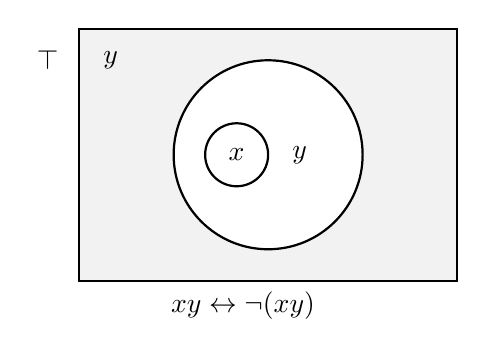
\begin{tikzpicture}[scale=0.8]
\draw[fill=gray!10,draw=black,thick](0,0)rectangle(6,4);
\draw[fill=white,draw=black,thick](3,2)circle(1.5 and 1.5);
\draw[fill=white,draw=black,thick](2.5,2)circle(0.5 and 0.5);
\draw(2.5,2)node{$x$};
\draw(3.5,2)node{$y$};
\draw(0.5,3.5)node{$\complementOf{y}$};
\draw(-0.5,3.5)node{$\top$};
\node[anchor=north] at (current bounding box.south) {$x \partOf \complementOf{y} \leftrightarrow \neg(x \overlaps y)$};
\end{tikzpicture}
\end{center}
{
\scriptsize 
This Venn-style diagram illustrates the equivalence incorporating complement, parthood and overlap:
Top $\top$ is the rectangle containing everything.
$x$ is a proper part of $y$.
The complement $\complementOf{y}$ of $y$ is emphasized as gray area.
$x$ shares no parts with $\complementOf{y}$.
}
\caption{A schematic illustration the equivalence incorporating Complement, Parthood \& Overlap}
\label{figure:SchematicEquivalenceOfCopmlementParthoodAndOverlap}
\end{figure}
Both equations follow directly from the definition of mereological difference by simple deduction, since $x \partOf \top$ is always true:
\begin{align}
\begin{split}
\complementOf{x} = \top - x
&\Leftrightarrow
\forall y(y \partOf \complementOf{x} \leftrightarrow x \partOf \top \wedge \neg(y \overlaps x))
\\&\Leftrightarrow
\forall y(y \partOf \complementOf{x} \leftrightarrow \neg(y \overlaps x))
\end{split}
\label{equation:CPO1}
\\
\begin{split}
x = \top - \complementOf{x} 
&\Leftrightarrow
\forall y(y \partOf x \leftrightarrow x \partOf \top \wedge \neg(y \overlaps \complementOf{x} ))
\\&\Leftrightarrow
\forall y(y \partOf x \leftrightarrow \neg(y \overlaps \complementOf{x} ))
\end{split}
\label{equation:CPO2}
\end{align}

A direct corollary is the identity of complement involution:
\begin{align}
\complementOf{(\complementOf{x})} = x
\end{align}
This identity is deduced by substitution of the equivalence above at \ref{equation:CPO1} and \ref{equation:CPO2}:
\begin{align}
\begin{split}
\complementOf{(\complementOf{x})} = T - \complementOf{x}
&\Leftrightarrow
\forall y (y \partOf \complementOf{(\complementOf{x})} \leftrightarrow \neg(y \overlaps \complementOf{x}))
\\&\Leftrightarrow
\forall y (y \partOf \complementOf{(\complementOf{x})} \leftrightarrow y \partOf x)
\\&\Leftrightarrow
\complementOf{(\complementOf{x})} = x
\end{split}
\end{align}

This property allows for a refinement of the definition for mereological difference, which again shows another similarity with set-theoretic difference:
\begin{align}
z = x - y = x \cdot \complementOf{y}
\end{align}
The proof is the same simple deduction as above:
\begin{align}
&\begin{split}
z = x - y
&\Leftrightarrow
\forall w (w \partOf z \leftrightarrow w \partOf x \wedge \neg (w \overlaps y))
\\&\Leftrightarrow
\forall w (w \partOf z \leftrightarrow w \partOf x \wedge w \partOf \complementOf{y})
\\&\Leftrightarrow
z = x \cdot \complementOf{y}
\end{split}
\end{align}

The notion of an universal top gives immediate rise to the question, whether a converse thing, an universal bottom, exists.
The universal bottom for parthood satisfies:
\begin{align}
&\exists \bot \forall x (\bot \partOf x)
&\qquad \text{(Bottom)}
\end{align}
An universal bottom renders the overlap relationship as defined at \ref{definition:Overlap} trivially true, thus the mereological product of two things can never be undefined.
In an algebraic sense, an universal bottom provides an absorbing element for the mereological product and a neutral element for the mereological sum:
\begin{align}
\bot &= \bot \cdot x = x \cdot \bot
\\
x &= \bot + x = x + \bot
\end{align}
Moreover, it makes mereological difference sound.
With an universal bottom the difference $x - x$ of only one thing is now possible:
\begin{align}
\begin{split}
z = x - x
&\Leftrightarrow
z = x \cdot \complementOf{x}
\\&\Leftrightarrow
\forall y (y \partOf z \leftrightarrow y \partOf x \wedge y \partOf \complementOf{x})
\\&\Leftrightarrow
z = \bot
\end{split}
\end{align}
The only thing, which is part of $x$ and its complement at the same time, is the universal bottom.
Given this fact, now complements of top and bottom can also be determined:
\begin{align}
\complementOf{\top}
&= \top - \top 
= \bot
\\
\complementOf{\bot}
&= \top - \bot 
= \top - \complementOf{\top} 
= \top \cdot \complementOf{(\complementOf{\top})}
= \top \cdot \top
= \top
\end{align}

However, the notion of an universal bottom or null thing is more controversial than the notion of an universal top \cite{DBLP:journals/dke/Varzi96}.

\ToDo{Outline why bottom is disputed. Perhaps, if bottom and atoms are assumed, bottom would be the only "real" atom.}


\subsection{Unrestricted Fusion}
\label{subsection:UnrestrictedFusion}

\subsection{Atomic Parts}
\label{subsection:AtomicParts}

\subsection{Mereology Theories}
\label{subsection:MereologyTheories}